\documentclass[12pt]{article}
\usepackage[a4paper, hmargin={2.8cm, 2.8cm}, vmargin={2.5cm, 2.5cm}]{geometry}
\usepackage{eso-pic} % \AddToShipoutPicture

\usepackage[utf8]{inputenc}
\usepackage[T1]{fontenc}
\usepackage{lmodern}
\usepackage[english]{babel}
\usepackage{cite}
\usepackage{amssymb}
\usepackage{amsfonts}
\usepackage{amsmath}
\usepackage{mathrsfs}
\usepackage{enumerate}
\usepackage{fullpage}
\usepackage[linkcolor=red]{hyperref}
\usepackage[final]{graphicx}
\usepackage{color}
\usepackage{listings}
\renewcommand*\lstlistingname{Code Block}
\definecolor{bg}{rgb}{0.95,0.95,0.95}

%caption distinct from normal text
\usepackage[hang,small,bf]{caption}
\usepackage{hyperref}

\hypersetup{
    colorlinks,%
    citecolor=black,%
    filecolor=black,%
    linkcolor=black,%
    urlcolor=black
}

\author{
  \texttt{Gruppe: 3D} \\
  \texttt{Mikkel Enevoldsen} \\[.4cm]
  \texttt{Kristian Høi} \\[.4cm]
  \texttt{Dominique F.N. Chancelier} \\[.4cm]
  \texttt{Carsten Jensen} \\[.4cm]
  Instruktor: Jesper Lundsgaard
  \vspace{8cm}
}

\title{
  \vspace{3cm}
  \Huge{Opgave 2} \\[.25cm]
  \large{Vurder brugergrænseflade}
  \vspace{.75cm}
}

\begin{document}

\AddToShipoutPicture*{\put(0,0){\includegraphics*[viewport=0 0 700 600]{includes/ku-farve}}}
\AddToShipoutPicture*{\put(0,602){\includegraphics*[viewport=0 600 700 1600]{includes/ku-farve}}}

%% Change `ku-en` to `nat-en` to use the `Faculty of Science` header
\AddToShipoutPicture*{\put(0,0){\includegraphics*{includes/ku-en}}}

\clearpage\maketitle
\thispagestyle{empty}

\newpage

%\tableofcontents %generate table of content

\thispagestyle{empty}

%\newpage
\pagestyle{plain}
\setcounter{page}{1}
\pagenumbering{arabic}

\section{Vis systemets tilstand}
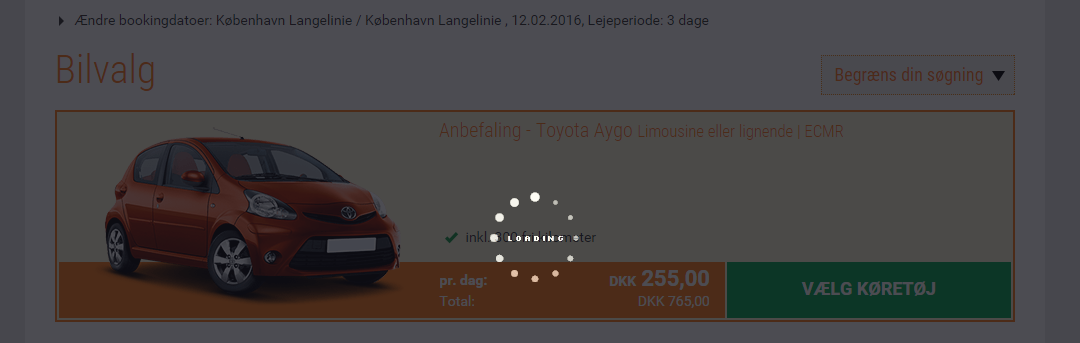
\includegraphics[scale=0.5]{img/Sixt_Loading}
\\
\\

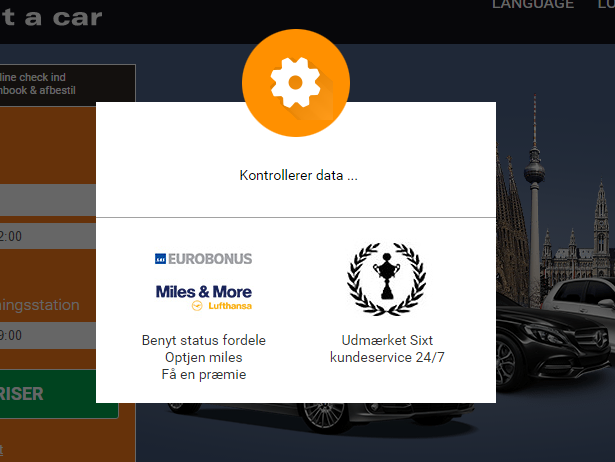
\includegraphics[scale=0.8]{img/Kontrollerer_Data}
\\
\\
Disse to billeder viser, at systemet klargøre bestillingssiden, og da denne proces tager mindre end fem sekunder, er det med bare en loading-besked. Dog er det inkonsistent at de ikke bruger samme loading-besked til begge processer.

\section{Tal brugeres sprog}
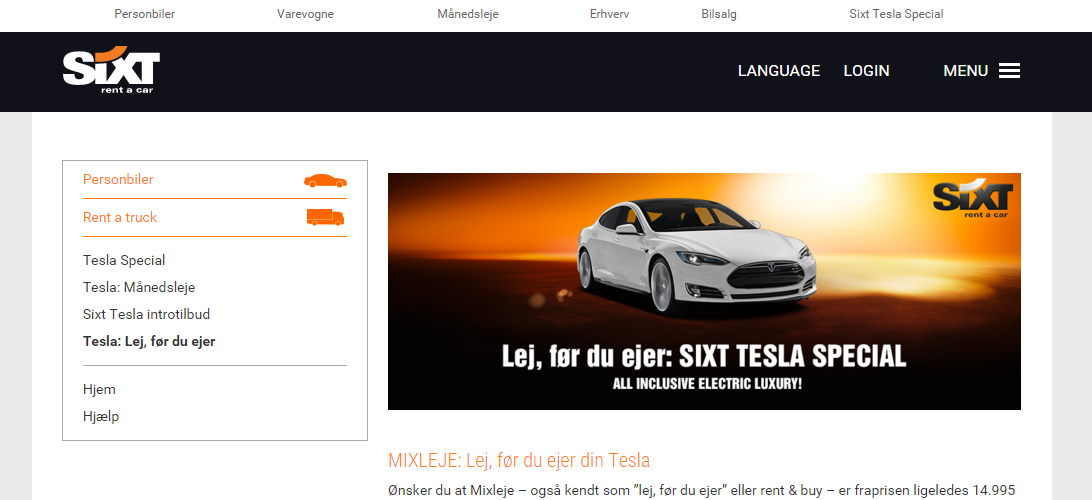
\includegraphics[scale=0.5]{img/Blande_Engelsk_Dansk}
\\
\\
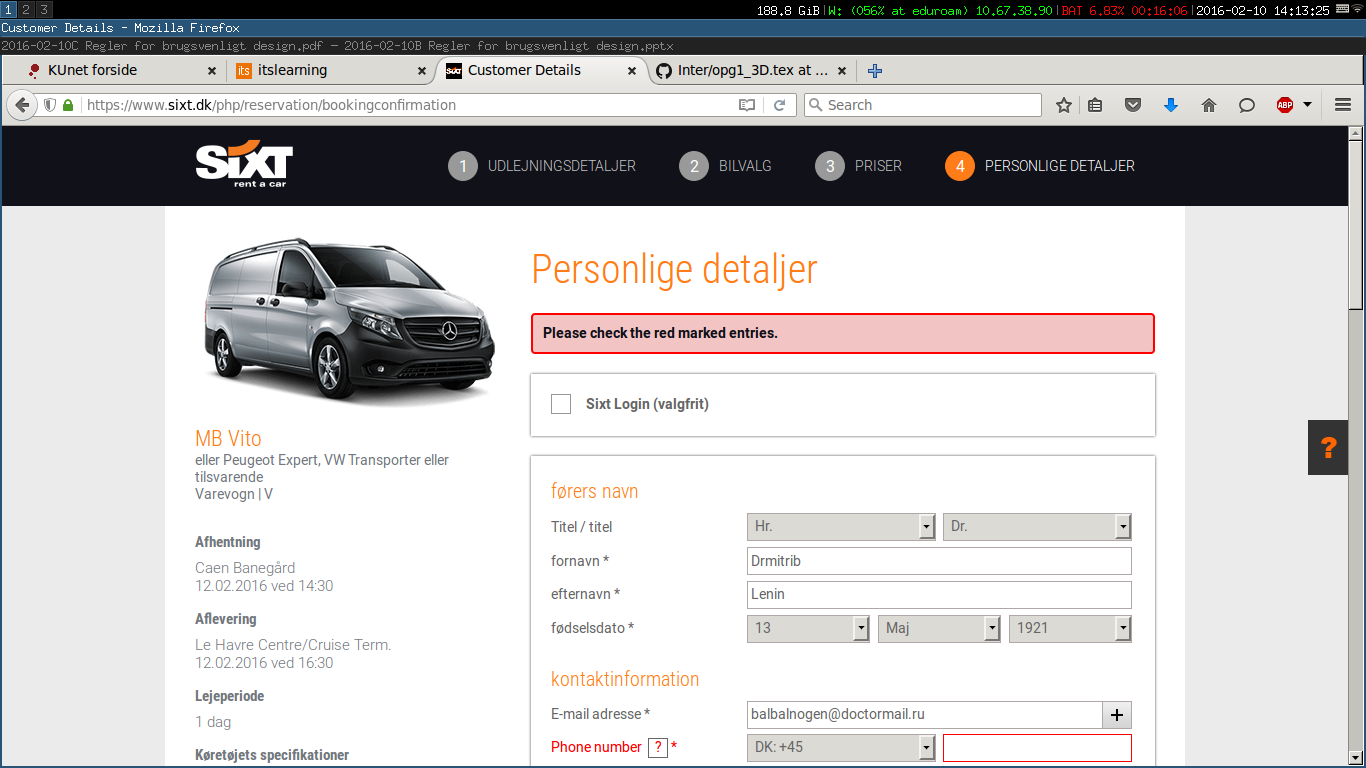
\includegraphics[scale=0.3]{img/CheckRedMarks}
\\
\\
Sixt.dk blander dansk og engelsk, og da vi er på et dansk domæne, må man forvente at teksten inklusiv fejlmeddelelser må være på dansk. Eksempelvis er "rent a truck" og "phone number" på engelsk, hvor resten af hjemmesiden er på dansk.

\newpage

\section{Lad brugeren bestemme}

På bestillingssiden er det ikke tydeligt markeret at annullere, dette kunne gøres med en annuller knap. Dette hæmmer markant brugerens frihed. Derudover har man heller ikke mulighed for at ændre sin bestilling undervejs. 


\section{Følg standarder}
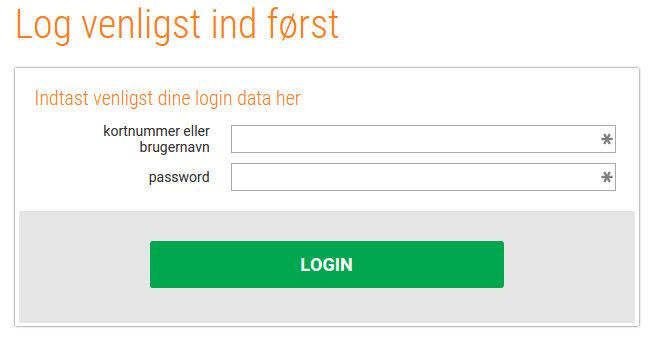
\includegraphics[scale=0.5]{img/standard}
\\
\\
Her følger Sixt.dk standarder og konventioner omkring login og brugeren mødes af en forventelig og genkendelig login-funktion.

\newpage

\section{Forebyg fejl}
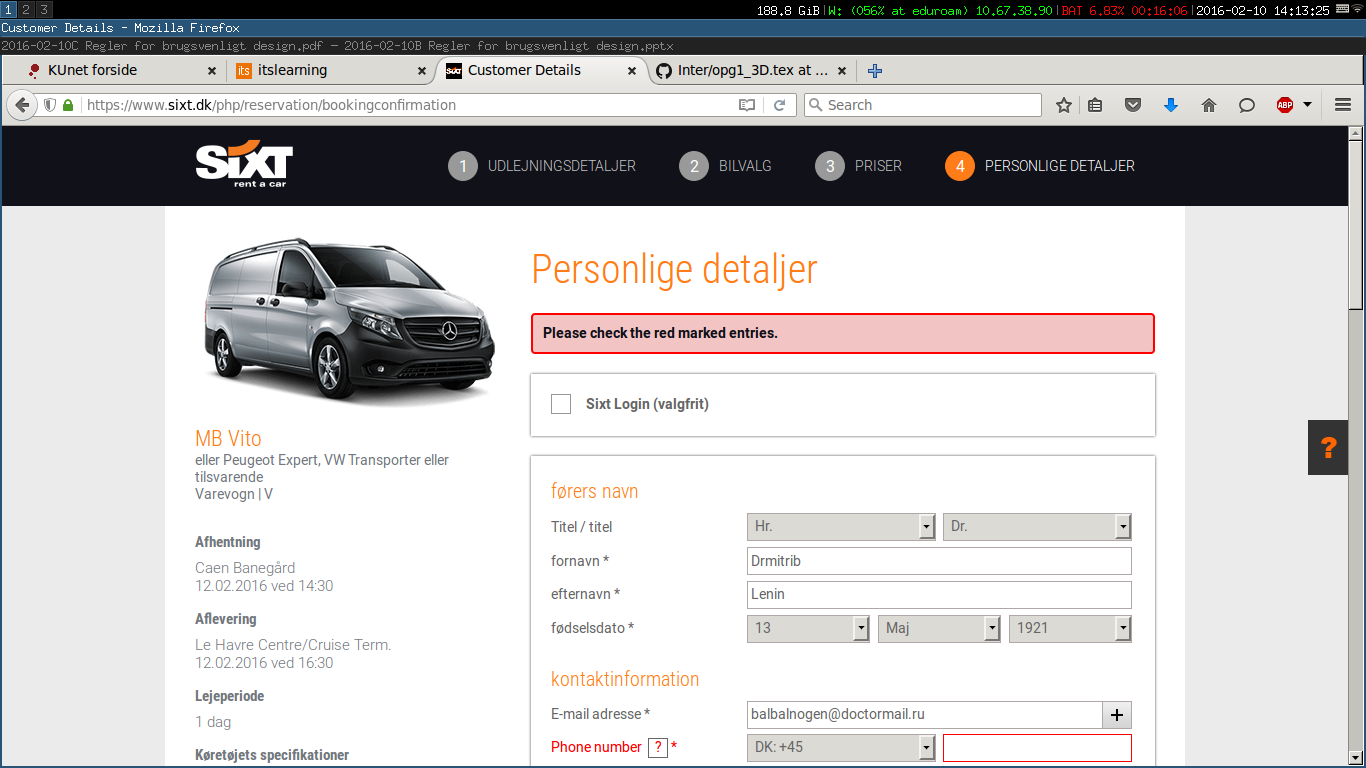
\includegraphics[scale=0.3]{img/CheckRedMarks}
\\
\\
Sixt.dk forebygger her en eller flere fejl i forbindelse med bestilling. I tilfælde af ugyldigt givet data giver markerer de manglende områder, og indikerer derved hvor den manglende information skal stå.
\\
\\

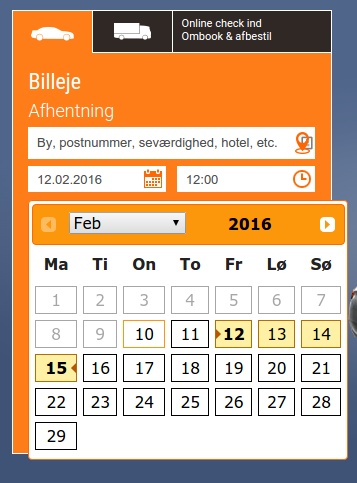
\includegraphics[scale=0.5]{img/calendar}
\\
\\
Ligesom før forebygges her fejl ved at letgøre datovalget. I samme instans kan afhentningsplaceringen kommenteres, da man ved indtastning af eksempelvis by, undervejs vil få muligheder i stedet for at skulle indtaste hele bynavnet.

\section{Støt hukommelse}

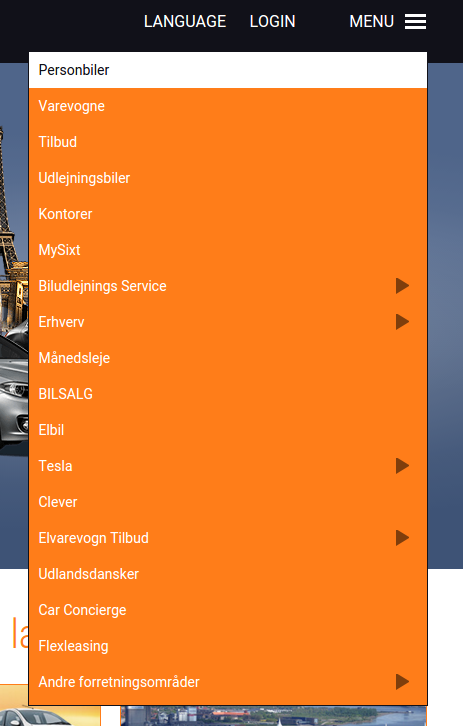
\includegraphics[scale=0.5]{img/menu}
\\
\\
I menuen vises hvad der må antages at være Sixt.dk's mest besøgte sider, hvilket gør det nemmere at navigere for brugeren. Derudover vises det åbent og er relativt nemt at annullere en bestilling, når den allerede indgået.

\section{Tilbyd fleksibel og effektiv betjening}

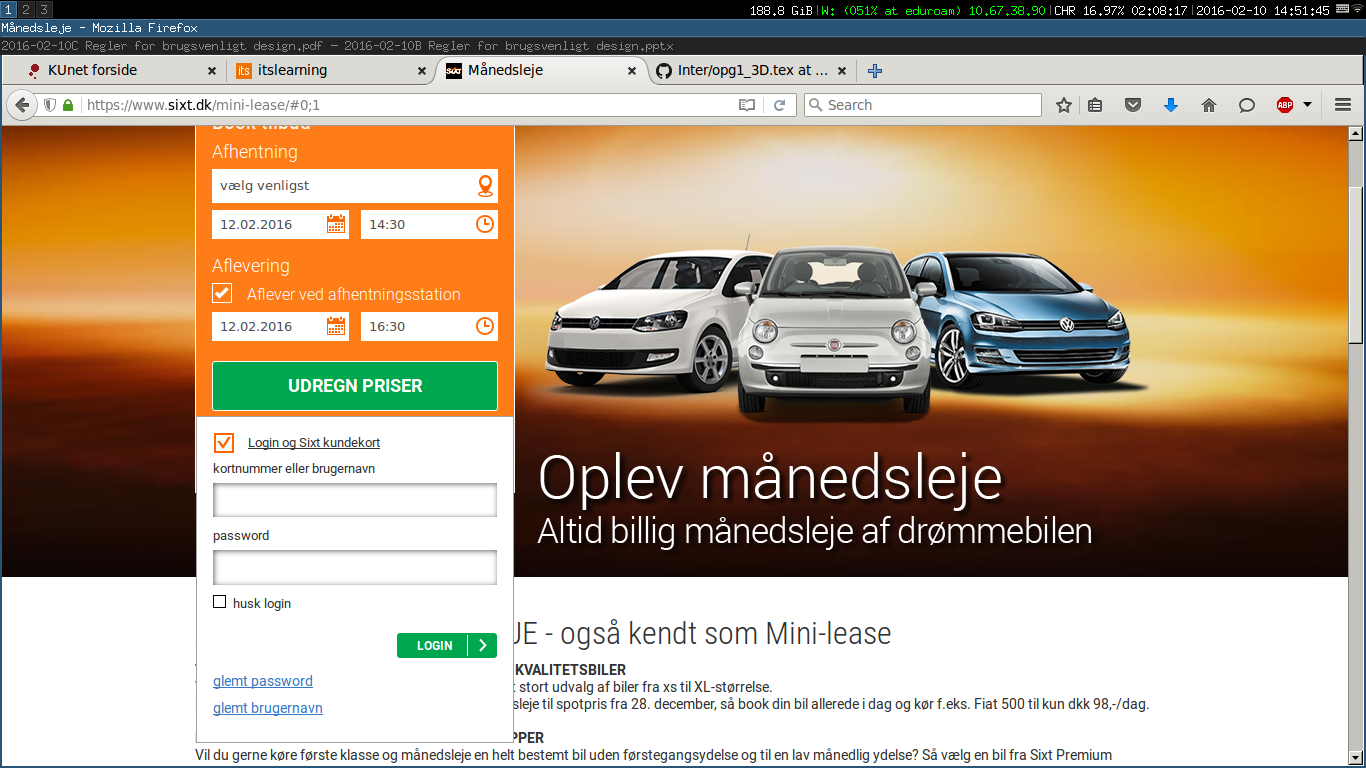
\includegraphics[scale=0.3]{img/PowerUser}
\\
\\
Ved hjælp af login-funktionen som vist herover, giver Sixt.dk muligheden for tidligere kunder gennem login at gemme deres oplysninger til fremtidigt brug. Placeringen af login under den store brik med "udregn priser" gør at nye brugere ikke tager hensyn til denne mulighed, og den er derved kun en aktuel for de øvede brugere. 

\section{Simplificér}

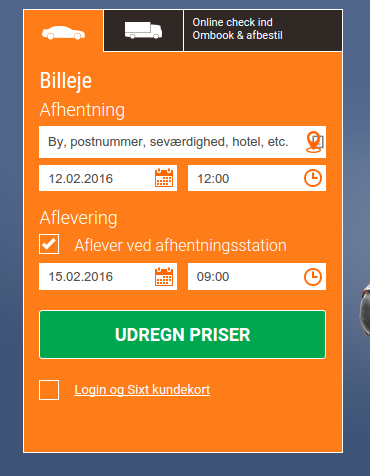
\includegraphics[scale=0.5]{img/simple}
\\
Prisudregningsprocessen som ses i billedet herover, er en godt simplificeret proces. Først kan der vælges mellem bil- eller varevognsleje, simplificeret ved et billede alle forstår. Derudover er selve afhentnings- og afleveringsstation også simplificeret som muligt.

\section{Hjælp, når der er problemer}

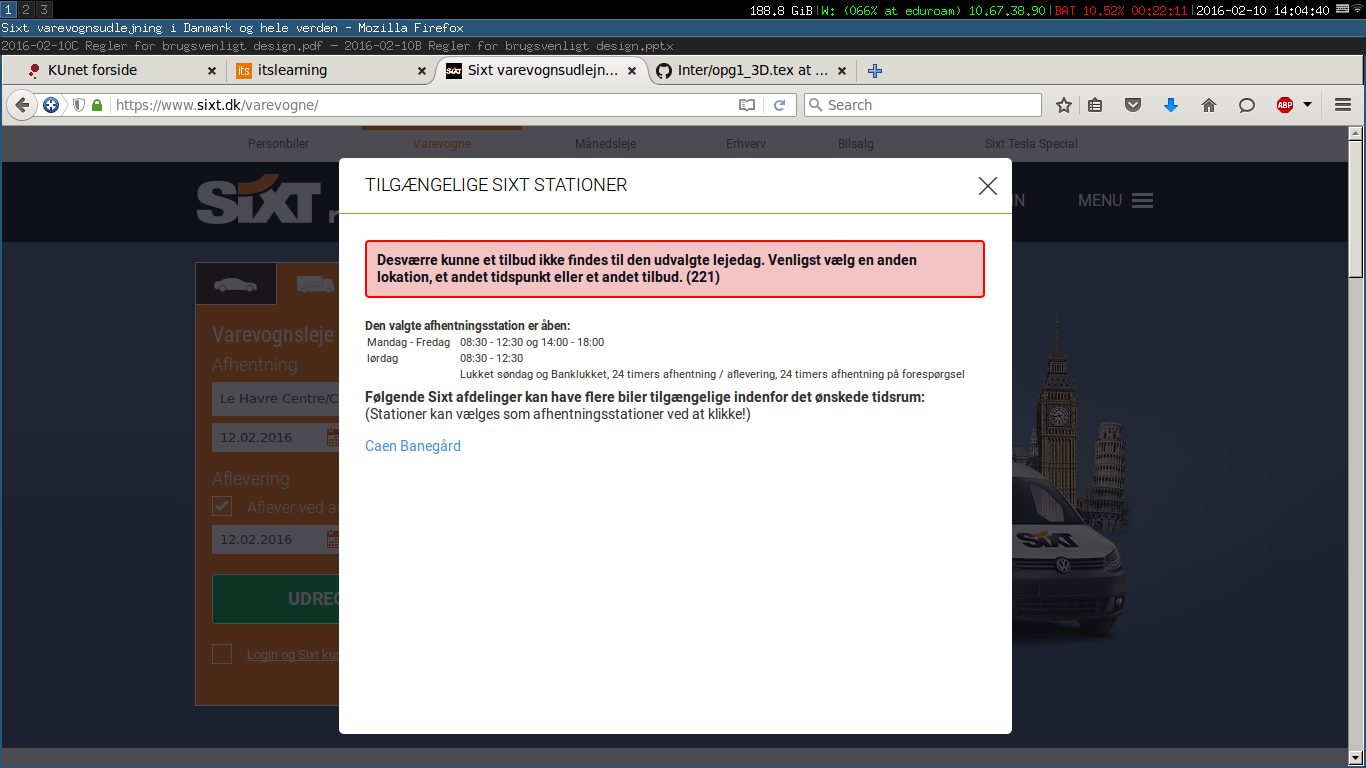
\includegraphics[scale=0.3]{img/Udlej222}
\\
\\
Her ses en fejlmeddelelse, hvor den afhentningsstation valgt ikke kunne finde et tilbud. Udover at give oplysninger omkring den valgte afhentningsstation, gives yderligere en station i nærheden, der vil kunne tilbyde en afhentning.

\section{Hjælp og dokumentation}

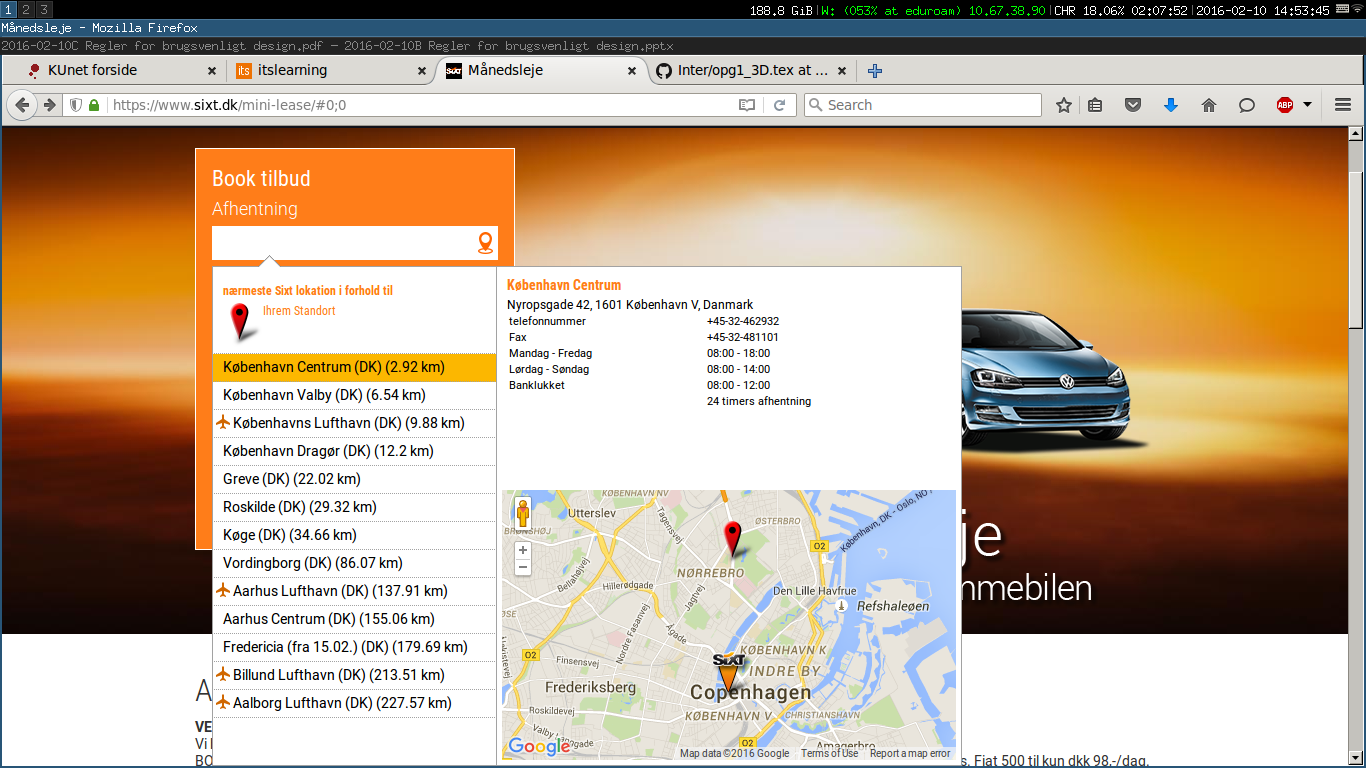
\includegraphics[scale=0.3]{img/NaermesteUdlejning}
\\
\\
I billedet ovenfor ses Sixt.dk's tilbud om at bruge GPS til at udregne den nærmeste afhentningsstation. Brugeren hjælpes altså i tilfældet af at vedkommende enten ikke kender en afhentningsstation eller ikke hvor han ønsker at hente den.

\end{document}
